% GUIDING QUESTIONS:
%
% What was the state of the art in this area, and what limitations exist?
%
% How does your project advance the state of the art, and why is it more
% effective than prior approaches?

\begin{frame}{Related Works}
    \huge
    \centering
    Related Works
\end{frame}

\begin{frame}{Aerial Networks}
    \begin{columns}
        \column{0.4\textwidth}
        \begin{itemize}
            \item Very little consideration of independent users as dynamic
            \item Consideration of probabilistic high-traffic areas \cite{drone-cells}
            \item Optimizing single-drone base-station trajectories \cite{drone-net-traj}
            \item Link to static base station \cite{drone-cells}
            \item Lacking differential-games perspective
        \end{itemize}

        \column{0.6\textwidth}
        \begin{figure}
            \centering
            \subfloat[{UAV base station serves traffic over its trajectory \cite[Fig. 1]{drone-net-traj}}]{
                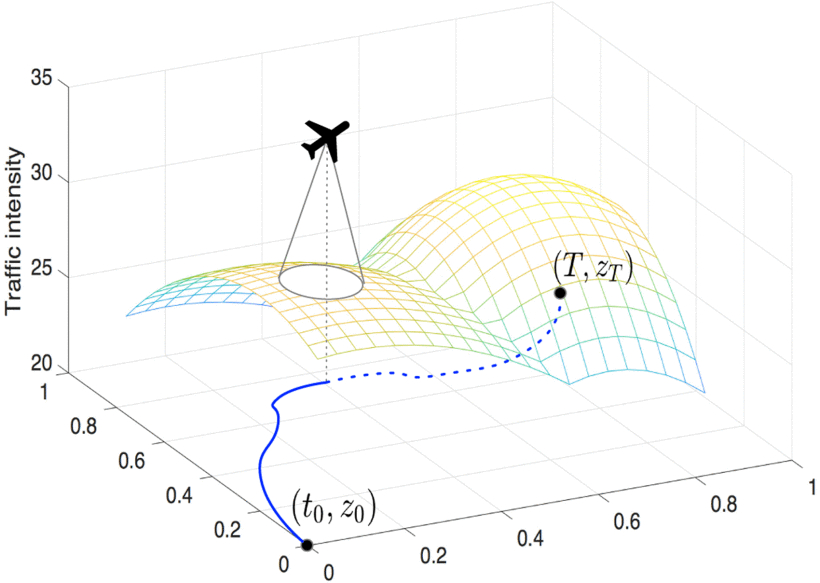
\includegraphics[width=0.45\linewidth]{assets/drone-trajectory.jpg}
            }
            \subfloat[{Drone assisted radio networks \cite[Fig. 1]{drone-cells}}]{
                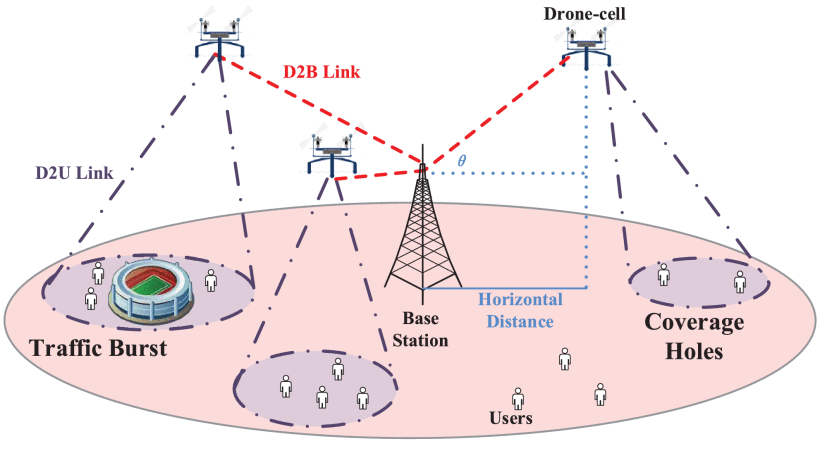
\includegraphics[width=0.45\linewidth]{assets/drone-cell-diagram.jpg}
            }
        \end{figure}
    \end{columns}

    % Current approaches to optimizing mobile aerial networks that tackle dynamic
    % traffic scenarios do not consider individual, moving users. These approaches
    % include generating trajectories for a drone travelling from point to point
    % while optimizing for high network service quality for users and minimized
    % control effort, \cite{drone-net-traj} or deployment of drone-based networks to
    % relieve transient traffic loads in high-usage zones. \cite{drone-cells}
    % Modelling network users as individuals who require highly reliable connections
    % is not considered. To the best of the author's knowledge, controls for aerial
    % network formation have not yet been studied using a differential games
    % approach.

    %To the best of the author's knowledge, there is also little research on the
    % application of differential games modelling to aerial networks for this reason.
    % One paper considering aerial networks \cite{drone-cells} applies
    % Hamilton-Jacobi equations (commonly used in differential games) to optimize the
    % trajectories of a UAV base station, but focuses on only a single UAV travelling
    % from a starting point to a destination. Another paper considering multi-drone
    % deployment scenarios applies particle swarm optimization (PSO) and
    % drone-iterated PSO (DI-PSO) \cite{drone-cells}. These approaches do not
    % consider dynamically moving users as individuals, but instead model users
    % according to a density with a Poisson distribution. \cite[III. A]{drone-cells}
    % Finally, \cite{pot-fields} uses spectral graph theory to form potential fields
    % that ensure individual agents in a multi-agent network remain within a
    % connected state while moving around.
\end{frame}

\begin{frame}{Differential Games}
    \begin{columns}
        \column{0.4\textwidth}
        \begin{itemize}
            \item 2P0S games in continuous time and space
            \item Common modelling approach to controls problems \cite[1118]{gt-modelling}
            \item Use the Hamilton-Jacobi-Isaacs equation to find saddle-point equilibrium (NE)
        \end{itemize}

        \column{0.6\textwidth}
        \begin{figure}
            \centering
            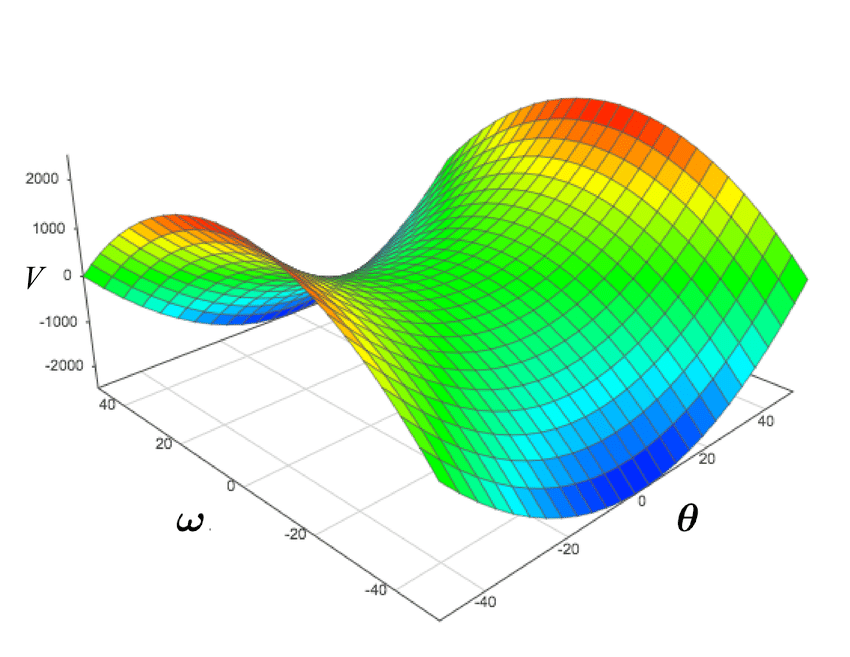
\includegraphics[width=0.6\linewidth]{assets/saddle.png}
            \caption{Saddle point equilibrium in 3D \cite{img:saddle}}
        \end{figure}
    \end{columns}
\end{frame}

\begin{frame}{Pursuit-Evasion Games}
    \begin{columns}
        \column{0.4\textwidth}
        \begin{itemize}
            \item Existing work is highly focused on capture \cite{mpme-sol, pe-intro,
                      pe-diff-speeds, stochastic-pe, discrete-pe, pe-env-constr}
            \item 2D capture games are analytically solved, but P-E pairings are
                  assigned in advance \cite{mpme-sol}
            \item Some consideration of 3D PE, but not multi-agent \cite{pe-diff-speeds}
        \end{itemize}

        \column{0.6\textwidth}
        \begin{figure}
            \centering
            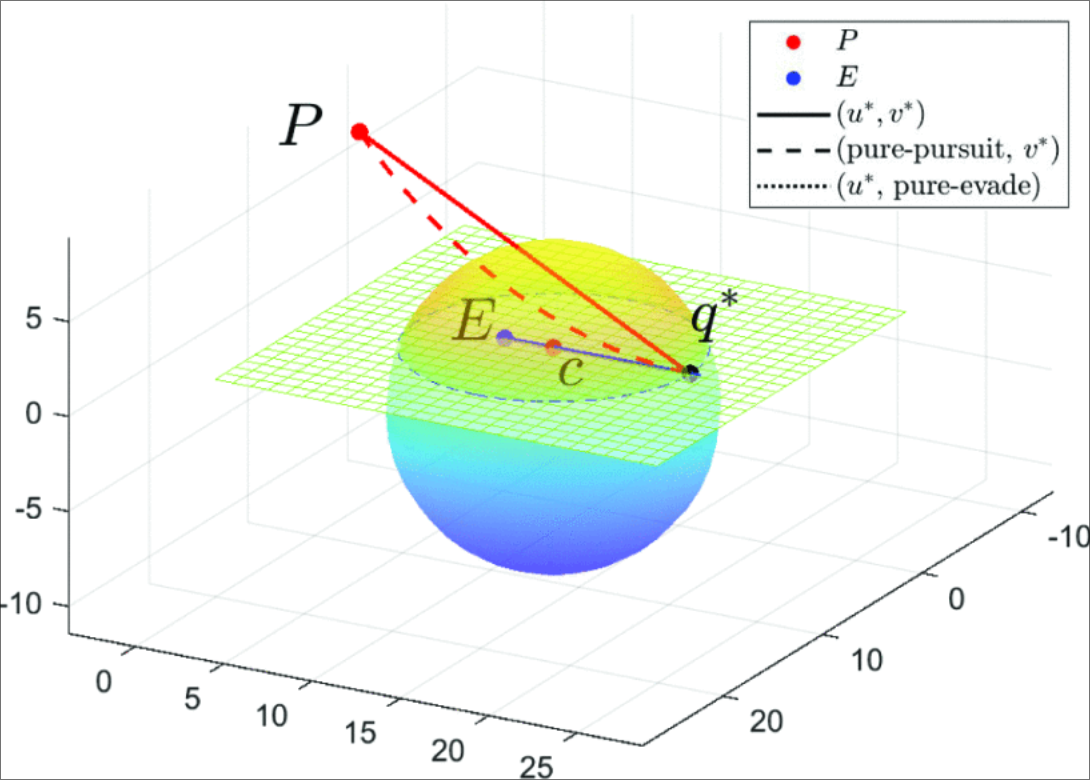
\includegraphics[width=0.6\linewidth]{assets/3d-pe.png}
            \caption{3D PE capture-based game \cite[Fig. 1]{pe-diff-speeds}}
        \end{figure}
    \end{columns}

    % Studies in the field of PE differential games focus primarily on the pursuing
    % team's capture of the evading team; either using point capture or a capture
    % radius \cite{mpme-sol, pe-intro, pe-diff-speeds, stochastic-pe, discrete-pe,
    %     pe-env-constr}. PE differential games considering point-capture and agents with
    % simple dynamics in 2D space have been analytically solved in \cite{mpme-sol},
    % yielding the closed-form saddle-point optimal controls for $n$ pursuers and $m$
    % evaders. However, the method proposed by \cite{mpme-sol} requires consideration
    % of all feasible assignments of pursuer-evader pairs in advance of the game's
    % start time to determine the optimal control assignments. The research in
    % \cite{pe-diff-speeds} extends 2D capture-based PE games into 3D space, where
    % evaders are constrained to a 2D "ground" plane and pursuers are free to
    % navigate in 3D space. The formulation in \cite{pe-diff-speeds} only considers a
    % single pursuer and a single evader. Several papers tackle other problems in
    % differential games, such as incomplete information \cite{discrete-pe,
    %     stochastic-pe} or dynamic constraints \cite{pe-env-constr}. There are no papers
    % to the knowledge of the author that consider a multi-agent PE game in which
    % pursuers coordinate to minimize a global cost without up-front computation of
    % pursuer-evader pairs \cite{mpme-sol} and without a focus on capture.
\end{frame}

\begin{frame}{Our Extensions}
    \begin{columns}
        \column{0.4\textwidth}
        \begin{itemize}
            \item Differential-game model of aerial network formation
            \item Admits a closed-form, saddle-point optimal control law for agents
            \item Multi-pursuer, multi-evader scenario in 3D instead of 1v1
            \item Differential game model with \textbf{cooperation} among pursuers
        \end{itemize}

        \column{0.6\textwidth}
        \begin{figure}
            \centering
            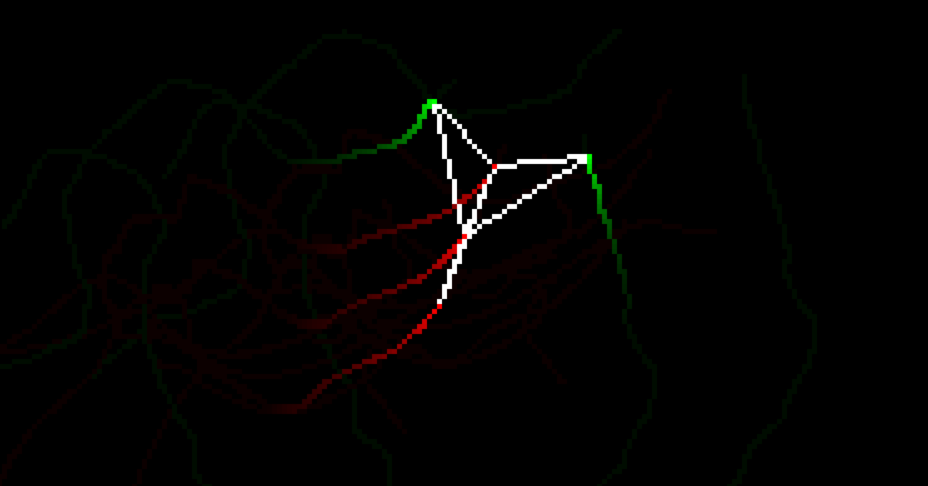
\includegraphics[width=0.8\linewidth]{assets/kite.png}
            \caption{Pursuers (red) and evaders (green) connected by an ad-hoc aerial network}
        \end{figure}
    \end{columns}
\end{frame}
